%% -*- coding: utf-8-unix -*-

\chapter{NetTesterの使いかた}
\label{chap:nettester-usage}

NetTesterによるテスト環境の構築方法やシステム要求、本PoCでの実際に使用し
た構成や機器・ソフトウェアの情報、基本的な使用方法について解説する。

 \section{NetTesterのデプロイ}
 \label{sec:nettester-deployment}

  \subsection{物理OpenFlowスイッチ}
  \label{sec:nettester-deploy-psw}

  % 物理OFSのデプロイ
  % - pica8 (OVS) の設定について
  %   - Portの設定(VLAN) : [L1PJTECH] 参照
  %   - \code{fail\_mode} の設定
  %     \url{https://docs.google.com/document/d/1yBn8S3DOhkuaVuVtUmwOeyvQxWm1v6_PfWTj3iDcx0U/}
  %   - inactivity probe の設定:
  %     調査: テスト環境でOFS(Pica8)-OFC(NetTester/Trema)の接続が切れる – NetTester
  %     \url{https://3.basecamp.com/3088280/buckets/867009/todos/218484578}
  %     \url{https://docs.google.com/document/d/1_-pLOXSOLutRb1_-tlcb_FwLCHq3Y7zQxp79_qXjDiM/}
  %     (そんなに重要じゃないけど一応)
  %   - 毎回ofsがcontrollerに繋いでくるのを待つ(10秒)のをどうにかしたい – NetTester
  %     https://3.basecamp.com/3088280/buckets/867009/todos/211396447

\ref{sec:nettester-model}節に示したとおり、NetTester は1台の物理OpenFlow
スイッチを利用して、テスト対象ネットワークへの接続をおこなう\footnote{1
台の物理OpenFlowスイッチを使用してテストトラフィックを ``distribute'' す
る。}。本節では物理OpenFlowスイッチの選択と設定について解説する。

    \paragraph{物理OpenFlowスイッチの要件と選択}
NetTesterが使用する物理OpenFlowスイッチには\tabref{tab:ofs-requirement}
の要件~\cite{l1pjpoc}が求められる。

\begin{table}[h]
 \centering
 \caption{OpenFlowスイッチ要件(OpenFlow/1.0)}
 \label{tab:ofs-requirement}
 \begin{tabular}{l|l}
  \hline
  分類 & 項目 \\
  \hline
  \hline
  Match  & In-Port \\ \cline{2-2}
         & VLAN ID \\ \cline{2-2}
         & Source/Destination MAC Address \\ \hline
  Action & Out-Port \\ \cline{2-2}
         & Push/Pop VLAN ID \\ \hline
  Other & Priority \\
  \hline
 \end{tabular}
\end{table}

本プロジェクトでは昨年度実施した \lopj の環境を継続しており、
\tabref{tab:psw-list}に示すOpenFlowスイッチを使用している。(2台の
OpenFlowスイッチを使用して Tester
set\footnote{\ref{sec:mgmt-and-tester-nw}節参照。} を2セット構築している。)

\begin{table}[h]
 \centering
 \caption{物理OpenFlowスイッチ}
 \label{tab:psw-list}
  \begin{tabular}{l|l|l}
   \hline
   Host name & Hardware & OS/Version \\
   \hline
   \hline
   OFS1 & Quanta T1048-LB9 & PicOS 2.5.2 / Revision 19975 \\
   OFS2 & Pica8 P-3290 & PicOS 2.2.1S3 / Revision 14775 \\
   \hline
 \end{tabular}
\end{table}

    \paragraph{物理OpenFlowスイッチの設定}
PicOSはOVS Mode (Open vSwitch)で使用する。物理スイッチ(PicOS OVS)では以
下の設定をおこなう。下記の設定事項については、PicOSマニュアルおよびOpen
vSwitchドキュメント~\cite{ovs-vswitchd-doc}も参照すること。
\begin{itemize}
 \item パッチとして使用する全ポートの設定~\cite{l1pjtech}
       \begin{itemize}
        \item VLANの操作をおこなうため、VLAN Mode を trunk として設定
              (\verb|vlan_mode=trunk|)する:
        \item テスト対象ネットワークで発生するブロードキャスト転送の抑制・
              STPへの干渉をさけるため、フラッディングを無効化
              (\verb|no-flood|)する。また、STPの無効化(\verb|no-stp|)を
              設定する。
       \end{itemize}
 \item 物理OpenFlowスイッチ(OVS Bridge)全体の設定
       \begin{itemize}
        \item BridgeでSTPを処理しない(\verb|stp_enable=false|)。
        \item OFCとの接続が切断された際にテスト対象ネットワークから届く
              トラフィックを処理しない
              (\verb|fail_mode=secure|)\footnote{\code{fail\_mode}には
              secureとstandaloneの2種類がある。Standaloneを指定した場合、
              OFS(OVS Bridge)はOFCとの接続がきれた際に独立したL2スイッチ
              (Learning Switch)として動作する。テスト対象ネットワークと
              の物理結線がある状態でL2スイッチとして動作してしまうと、テ
              スト対象ネットワークをまきこんでL2ループが発生してしまうた
              め注意が必要である。}\footnote{PicOSでは、PicOSバージョン
              が異なると(PicOS上のOVSのバージョンが同一でも)OVSの
              \code{fail\_mode}デフォルト設定が異なっているため注意が必
              要である。利用する場合は明示的に\code{fail\_mode=secure}を
              設定すること。}。
        \item NetTesterでは、利用する物理OpenFlowスイッチのDPIDを指定で
              きる(\ref{sec:nettester-envvar}節)。PicOSでは
              \lstref{lst:psw-openflow-config}のようにOFC(NetTester
              Controller)およびDPIDを設定する\footnote{PoCでは物理
              OpenFlowスイッチのDPIDを\code{0x1}としている。}。
        \item (Optional) OFSとOFCの接続に時間がかかる場合、OVSの
              \verb|max_backoff|\footnote{OFSがOFCに接続を試みる際のイン
              ターバルの指定。ミリ秒単位で指定でき、最小は1秒(
              \code{max\_backoff=1000})である。}値を調整する
              \cite{ovs-backoff-doc}。
        \item (Optional) OFSとOFCとの接続がタイミングにより切断されるな
              どの現象がある場合には、
              \verb|inactivity_probe|\footnote{OFS-OFC間接続の中断時間
              (idle time)の最大値。Inactivity probe で設定した時間
              OFS-OFC間での通信が発生していない場合、OFSはOFCへprobeを送
              信する(OFCがprobeに応答しない場合はコネクション切断と見な
              して再接続をおこなう)。ミリ秒単位で指定する。0を指定するこ
              とで設定が無効化される。} の値を調整する。
       \end{itemize}
\end{itemize}

\begin{lstlisting}[language=sh,caption=物理スイッチのOpenFlow設定,label=lst:psw-openflow-config]
ovs-vsctl set bridge br0 other-config:datapath-id=0000000000000001
ovs-vsctl set-controller br0 tcp:[NetTester Server Mgmt IP]:6653
\end{lstlisting}

  \subsection{NetTester Server の構成選択}
  \label{sec:nettester-server-deploy-pattern}

  % NetTesterモデルの制約とサーバ構成の選択肢
  % - 必要なNIC
  % - ベアメタル
  % - KVM による仮想化, その場合のNIC設定

NetTesterサーバは物理OpenFlowと物理リンクで直結される必要がある。サーバ
の構成方法として、ベアメタル構築する場合と仮想マシンで構築する場合の注意
事項について解説する。

\paragraph{ベアメタル構成}
NetTesterサーバをベアメタルで構成する場合は
\figref{fig:nettester-deploy-baremetal}のようになる。
\ref{sec:nettester-model}節に示したとおり、NetTesterサーバと物理スイッチ
(PSW)間は物理リンクで直結される必要がある。また、OpenFlowチャネルや
NetTester-PSW間の制御・管理通信のために、NetTesterサーバとPSWは管理ネッ
トワークを介して通信をおこなう。
\begin{figure}[h]
 \centering
 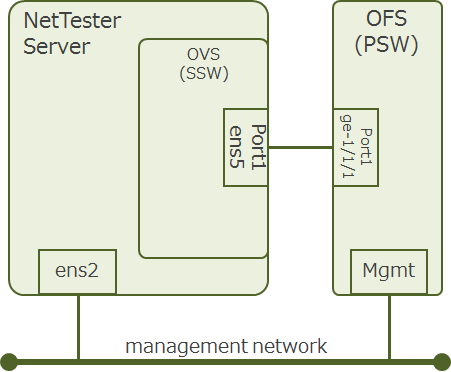
\includegraphics[scale=0.6]{img/nettester-deploy-baremetal.png}
 \caption{ベアメタル構成}
 \label{fig:nettester-deploy-baremetal}
\end{figure}

\paragraph{仮想マシン構成}
NetTesterサーバを仮想マシンとして構成する場合は
\figref{fig:nettester-deploy-vm}のようになる。管理ネットワークについては
ベアメタル構成の場合と同様にL2/L3でPSWとのコネクティビティがとれればよい。
NetTester(SSW)-PSW間の接続については、ホストOS側で物理ポート(リンク)を
NetTesterサーバ(VM)へ直結させる必要がある。SSW-PSW間はOFC(NetTester)によっ
て制御するため、ハイパーバイザ側ではL2以上の制御はおこなわない。パススルー
あるいはプロミスキャスモードで接続する。

\begin{figure}[h]
 \centering
 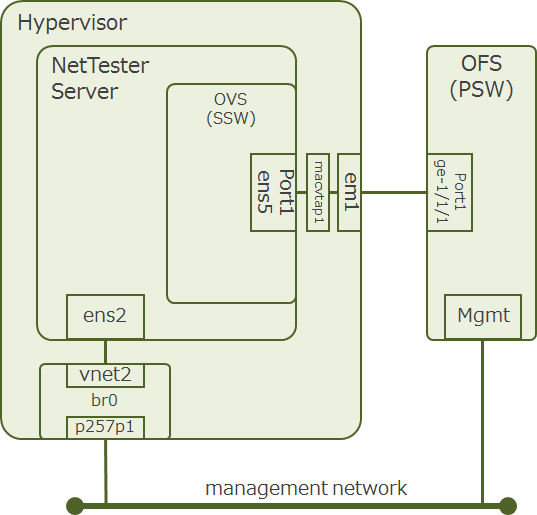
\includegraphics[scale=0.6]{img/nettester-deploy-vm.png}
 \caption{仮想マシン構成}
 \label{fig:nettester-deploy-vm}
\end{figure}

本プロジェクトは仮想マシン構成を採用した。PoCでは
\tabref{tab:server-spec}に示すサーバを使用している。SSW-PSW間接続では、
ハイパーバイザ(KVM Host)が持つ物理NICを直接仮想マシンに接続
(\code{macvtap/passthrough})させる(\lstref{lst:kvmconf-psw-port})。管理
ネットワークについては bridge 接続でよい(他のVMやハイパーバイザとL2で接
続する, \lstref{lst:kvmconf-mgmt-port})。

\begin{table}[hb]
 \centering
 \caption{NetTesterサーバ情報}
 \label{tab:server-spec}
 \begin{tabularx}{\linewidth}{l|X|X}
  \hline
  Host & OS & Virtualization \\
  \hline
  \hline
  \shortstack[l]{Hypervisor\\(KVM Host)}
    & \shortstack[l]{Ubuntu 14.04.5 LTS\\(GNU/Linux 3.16.0-30-generic x86\_64)}
    & \shortstack[l]{qemu-kvm/2.0.0+dfsg-2ubuntu1.25,\\libvirt/1.2.2-0ubuntu13.1.17} \\
  \hline
  \shortstack[l]{NetTester Server\\(VM)}
    & \shortstack[l]{Ubuntu 16.04.1 LTS\\(GNU/Linux 4.4.0-31-generic x86\_64)}
    & \\
  \hline
 \end{tabularx}
\end{table}

\begin{lstlisting}[language=xml,caption=PSW接続用ポート設定,label=lst:kvmconf-psw-port]
<interface type='direct'>
  <mac address='52:54:00:12:56:0e'/>
  <source dev='em1' mode='passthrough'/>
  <target dev='macvtap1'/>
  <model type='virtio'/>
  <alias name='net1'/>
  <address type='pci' domain='0x0000' bus='0x00' slot='0x05' function='0x0'/>
</interface>
\end{lstlisting}
\begin{lstlisting}[language=xml,caption=管理ポート設定,label=lst:kvmconf-mgmt-port]
<interface type='bridge'>
  <mac address='52:54:00:64:ee:38'/>
  <source bridge='br0'/>
  <target dev='vnet2'/>
  <model type='virtio'/>
  <alias name='net0'/>
  <address type='pci' domain='0x0000' bus='0x00' slot='0x02' function='0x0'/>
</interface>
\end{lstlisting}


  \subsection{NetTester Server のソフトウェア構成}
  \label{sec:nettester-server-software}

  % 必要なソフトウェア(package)とインストール
  % - 基本的なパッケージ
  %   - open vswitch
  %   - ruby, rubyenv
  %   - Git
  %   - Build-Essentials
  % - OSの設定
  %   - sudoers secure\_path

    \paragraph{NetTesterを使用するために必要なソフトウェア}
\nettester を使用するための必須ソフトウェアとPoCで使用したバージョンにつ
いて\tabref{tab:nettester-software-stack}に示す。使用するソフトウェアの
導入にあたっての注意事項を以下に示す。
\begin{itemize}
 \item \tabref{tab:nettester-software-stack}以外に必要な一般的な開発ツー
       ル等については Build Essential~\cite{build-essential-doc}などで導
       入しておく\footnote{\code{sudo apt install build-essential}}こと。
 \item NetTesterで使用するRuby package(gem)はbundlerで自動的にインストー
       ルされる。GemについてはNetTesterリポジトリ内 \code{Gemfile}等を参
       照すること。
 \item Rubyについてはrbenv~\cite{rbenv}などで複数のrubyバージョンを管理
       する環境でもよい。
 \item NetTesterはバックエンドで\code{ip}コマンドを使用してNetwork
       Namespaceの操作をおこなっている\footnote{正確にはNetTesterが利用
       しているTrema/Phutが\code{ip}コマンドを使用している。
       \ref{sec:phut_basics}節参照。}。このときroot権限が必要になり
       \code{sudo}を使用して実行する。\code{sudo}利用にあたって
       \code{PATH}に関するエラーが発生する場合は\code{sudo}設定ファイル
       (\code{/etc/sudoers})の\code{secure\_path}設定を修正すること。
\end{itemize}

  \begin{table}[H]
   \centering
   \caption{NetTester Serverのソフトウェア構成}
   \label{tab:nettester-software-stack}
   \begin{tabularx}{\linewidth}{l|l|X}
    \hline
    Software & Version (PoC) & Notes \\
    \hline
    \hline
    OS (Linux) & \shortstack[l]{Ubuntu 16.04 (GNU/Linux 4.4.0),\\ \tabref{tab:server-spec}参照} & Linux Network Namespace が使用できること。 \\
    \cline{1-2}
    iproute2 & 4.3.0 & \\
    \hline
    ethtool & 4.5 & NIC オフロード機能操作 \\
    \hline
    Git & 2.7.4 & \\
    \hline
    Open vSwitch & 2.5.0 & SSWとして使用する。\tabref{tab:ofs-requirement}を満たすこと。 \\
    \hline
    Ruby & 2.3.1p112 & 2.0以上が必要。2.3以上を推奨。\\
    \hline
   \end{tabularx}
  \end{table}

    \paragraph{Open vSwitch(SSW)の設定}
NetTesterサーバ上のソフトウェアスイッチは、NetTester起動時に都度
NetTesterが設定をおこなうため、事前に設定等をおこなう必要はない。
NetTesterを起動すると、\ref{sec:nettester-model-restriction}節に示した
DPIDでOpen vSwitchのブリッジが作成され、OFCとの接続設定がおこなわれる。

    \paragraph{NICのハードウェアオフロード機能操作}
    % trunkを使ってTCP通信するとおかしくなる – NetTester
    % https://3.basecamp.com/3088280/buckets/867009/todos/368843648
    % Netns Checksum Offload 機能実装 – NetTester
    % https://3.basecamp.com/3088280/buckets/867009/todos/370752297
NetTesterをつかったテストシナリオの実装・テスト実行の際、以下の条件で正
しく通信がおこなえない問題がおきた。事象としては、テスト用ノードが生成し
ているTCPパケットのチェックサムが incorrect となっていた。
\begin{itemize}
 \item テスト用ノードをテスト対象ネットワークに trunk port で接続させる。
       (OVSでVLAN Tagを操作する。)
 \item テストトラフィックとしてTCP通信をおこなう。
       \begin{itemize}
        \item SYN/FINフラグがついたトラフィックについては問題が発生しな
              い。(TCPで特定のフラグがついたパケットで問題がおきる。)
        \item ICMP通信については問題が発生しない。
       \end{itemize}
\end{itemize}
事象の根本的な原因究明はできていない。ワークアラウンドとして、NetTester
でテスト用ノード(Netns)を生成した際、ノード用のNIC(veth)でチェックサム計
算のハードウェアオフロードを無効化している~\cite{net-tester-pr7}。

  \subsection{テストシナリオ (net-tester/examples) のインストール}
  \label{sec:deploy-test-cenario}
  % 必要なソフトウェア(package)とインストール
  % - 基本的なパッケージ
  %   - テストシナリオでつかうもの (nc, dnsmasqなど)

  % テストシナリオで使うツール(package)の解決 – NetTester
  % https://3.basecamp.com/3088280/buckets/867009/todos/327898933

本プロジェクトでは、NetTester を使用したネットワークのテストシナリオを
\nettesterex として整備している。

テストシナリオをインストールする場合は\lstref{lst:install-scenario}の手
順を実行する。テストシナリオの中でNetTesterはテスト用ノード操作をおこな
う際に使用するツールのひとつとなるため、bundlerにより自動的にインストー
ルがおこなわれる。NetTester以外にテストシナリオ(Cucumberで記述)内で使用
するruby gemsについても、リポジトリ内\code{Gemfile}等で管理される。

\begin{lstlisting}[language=sh,caption=テストシナリオのインストール,label=lst:install-scenario]
git clone https://github.com/net-tester/examples.git
cd examples
bundle install --binstubs --path=vendor/bundle
\end{lstlisting}

このほかに、テストシナリオでは、NetTesterを使って生成・配置したテスト用
ノードの上で、さらにテストトラフィックを生成し end-to-end の通信状況を見
ていくためのツールが必要になる。PoCテストシナリオでは
\tabref{tab:tools-for-scenario}に示すツールを使用している。2017年1月時点
で、テストシナリオ内で使用する(bundlerで管理できるruby packageではない)
ツールについては統一した管理はできていない。テストシナリオ中で使用するツー
ルについては、手動で別途インストールする必要がある。

\begin{table}[h]
 \centering
 \caption{PoCテストシナリオ内で使用するツール}
 \label{tab:tools-for-scenario}
 \begin{tabular}{l|l|l}
  \hline
  Tool(package) & Version & テストシナリオ内での使いかた \\
  \hline
  \hline
  netcat(\code{nc}) & 1.105 & 汎用/簡易TCPサーバとして使用 \\
  dnsmasq & 2.75 & DNS通信テスト用の軽量DNSサーバとして使用 \\
  curl & 7.47.0 & HTTP(HTTPS)アクセス用クライアントとして使用 \\
  openssl & 1.0.2g & HTTPSサーバで使用 \\
  openssh & 7.2p2 & SSHサーバ/クライアントで使用 \\
  \hline
 \end{tabular}
\end{table}

  \subsection{NetTesterのインストール}

テストシナリオを中心にネットワークのテストを開発する場合は
\ref{sec:deploy-test-cenario}節のとおり、テストプロジェクト(リポジトリ)
が使用するツールのひとつとしてNetTesterが含まれる。

NetTesterを直接(単体で)使用して簡単なテスト操作をおこなうこともできる。
そうした場合には\lstref{lst:install-nettester}の手順でNetTester単体での
インストールをおこなう。

\begin{lstlisting}[language=sh,caption=NetTesterのインストール,label=lst:install-nettester]
git clone https://github.com/net-tester/net-tester.git
cd net-tester
bundle install --binstubs --path=vendor/bundle
\end{lstlisting}

 \section{基本的な使い方}
 \label{sec:basic-usage}

  \subsection{NetTesterが使用する環境変数}
  \label{sec:nettester-envvar}
  % 環境変数の設定
  % - ``DEVICE``
  %   - 調査:セグメントローカルの試験がとおらない – NetTester
  %     \url{https://3.basecamp.com/3088280/buckets/867009/todos/259184454}
  %   - ネットワークデバイスと dpid を rake に渡せるようにする – NetTester
  %     \url{https://3.basecamp.com/3088280/buckets/867009/todos/214833956}
  % - expectacle 関連についてはappendixにうつすか。

NetTesterは以下の2つの環境変数を使用する。
\begin{description}
 \item[\code{DEVICE}] NetTesterサーバ上で、SSW-PSW間を接続するために使用
            するNICを指定する。
 \item[\code{DPID}] 物理OpenFlowスイッチ(PSW)のDatapath IDを指定する。
\end{description}

\figref{fig:nettester-deploy-vm}の場合は\code{DEVICE=ens5}、
\code{DPID=0x1}となる。テストシナリオ(NetTester Examples)では\code{rake}
により複数テストシナリオの一括実行(回帰テスト)を実行できる。\code{rake}
実行時には次のように環境変数を指定して実行する。
\begin{lstlisting}
rake DEVICE=ens5 DPID=0x1 cucumber
\end{lstlisting}

この他に、テスト対象ネットワーク機器操作のために使うツール
(\ref{sec:expectacle}節)でも、テストシナリオ実行の際に環境変数を使用する
ので注意すること。

  \subsection{NetTester APIの基礎}
  \label{sec:nettester-api-basics}
  % NetTesterでad-hocなテスト作業を拡張する - Qiita
  % \url{http://qiita.com/corestate55/items/d6a8cdc03de09a46877c}

NetTesterを使った処理の基本的な流れと、APIの基本的な使用方法を例をもとに
解説する。

\paragraph{サンプル環境構成}

いま\figref{fig:nettester-basic-example}のように、テスト対象ネットワーク
にあるふたつのL2スイッチ(L2SW)に、1台ずつテスト用ノードを接続してテスト
作業を実施すると仮定する。このとき、テスト用ノードの生成および配置・接続
はNetTesterを使用しておこなう。また、テスト用ノードで実施するテスト作業
はPry~\cite{pry}を使用してad-hocに(手動で)実施する。

これをNetTester APIを用いて実装すると
\lstref{lst:nettester_basic_example}のようになる\footnote{このスクリプト
は解説用にパラメタ設定などを冗長に記載している。実際にテストシナリオ等を
実装する場合は、より無駄のない形で記述することができる
(\ref{sec:test-parameter-management}節参照)。}。
% TODO: FactoryGirlの話とかへの参照をいれたい

\begin{figure}[h]
 \centering
 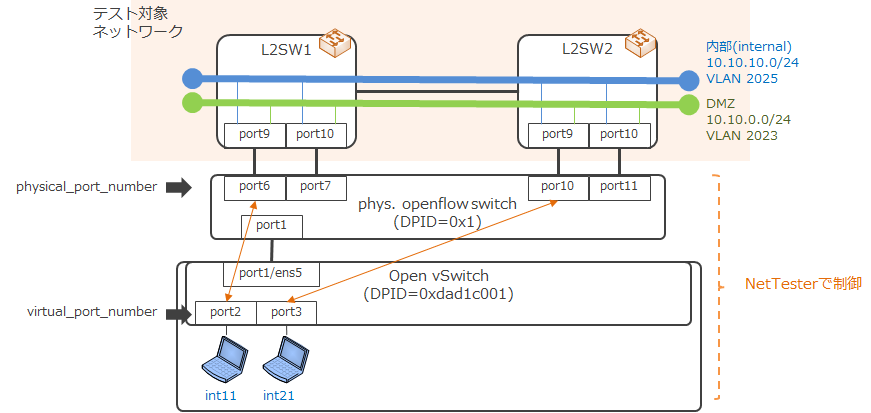
\includegraphics[scale=0.75]{img/nettester-basic-example.png}
 \caption{NetTester利用例(構成図)}
 \label{fig:nettester-basic-example}
\end{figure}

\begin{lstlisting}[caption=NetTester基礎,label=lst:nettester_basic_example]
#!/usr/bin/env ruby
# frozen_string_literal: true

require 'net_tester'
require 'pry'

# parameter definition
nwdev = 'ens5'
pss_dpid = 0x1
mac_base = '00:ba:dc:ab:1e:'

p '# run net_tester'
NetTester.run(network_device: nwdev,
              physical_switch_dpid: pss_dpid)
p '# wait ssw/psw connection'
sleep 10

p '# Create host11 in internal segment (ip:10.10.10.7, vlan:2025)'
host11 = NetTester::Netns.new(name: 'host11',
                              mac_address: mac_base + '01',
                              ip_address: '10.10.10.7',
                              netmask: 24,
                              gateway: '10.10.10.254',
                              virtual_port_number: 2,
                              physical_port_number: 6,
                              vlan_id: 2025)

p '# Create host21 in internal segment (ip:10.10.10.9, vlan:2025)'
host21 = NetTester::Netns.new(name: 'host21',
                              mac_address: mac_base + '02',
                              ip_address: '10.10.10.9',
                              netmask: 24,
                              gateway: '10.10.10.254',
                              virtual_port_number: 3,
                              physical_port_number: 10,
                              vlan_id: 2025)

# into pry console
binding.pry

# cleanup
NetTester.kill
\end{lstlisting}

    \paragraph{NetTesterによるテスト操作の流れ}
NetTesterを使ったネットワークのテスト操作は次のステップで実装する。
\begin{enumerate}
 \item NetTesterを起動する
       \begin{itemize}
        \item \verb|NetTester.run| (引数については
              \ref{sec:nettester-envvar}節参照)
        \item 起動すると、SSWの設定とOFCの起動をおこなう。
              \lstref{lst:nettester_basic_example}ではOFC起動後にSSW/PSW
              の接続を待つために\code{sleep}を設定している。
       \end{itemize}
 \item NetTesterでテスト用ノードを生成する
       \begin{itemize}
        \item \verb|NetTester::Netns.new| によって Network Namespace を
              使ったテスト用ノードを生成する。(詳細については
              \ref{sec:phut_basics}節参照)
        \item 生成と同時にテスト対象ネットワークへの配置(パッチ接続)をお
              こなう。引数\verb|virtual_port_number|および
              \verb|physical_port_number|は「パッチ」の両端点となるポー
              ト番号をあらわしている。ここで指定された端点情報をもとに、
              NetTesterはOpenFlowスイッチ(PSW, SSW)にフロールールを設定
              する。
        \item \figref{fig:nettester-basic-example}で、L2SW側のテスト用ノー
              ド接続ポートはTrunk Port (vlan tagged port)になっている。
              そのため、\verb|vlan_id|引数でテスト用ノードが生成するトラ
              フィックにVLAN Tagを指定している。
       \end{itemize}
 \item 生成したテスト用ノード上で作業をおこなう
       \begin{itemize}
        \item \verb|NetTester::Netns#exec| (後述)
       \end{itemize}
 \item NetTesterを終了する
       \begin{itemize}
        \item \verb|NetTester.kill|
        \item NetTesterが生成したSSW, テスト用ノードなどを削除する。テス
              ト用ノード(\verb|NetTester::Netns|)の実態は network
              namespace である。そのため、NetTester側で適切な終了(削除)
              処理がおこなわれない場合、OS上にこれらの設定が残りつづけて
              しまう。他のテストシナリオ実行時に同名のnamespaceを作成し
              ようとするとエラーになるため注意が必要である。
       \end{itemize}
\end{enumerate}

テスト用ノード上での操作については、このスクリプトではpryによるインタラ
クティブシェル上での操作となる。生成したテスト用ノード上(テスト用ノード
のnamespace上)でコマンドを実行することでテスト作業をおこなう。テスト用ノー
ド上でのコマンド実行には\verb|NetTester::Netns#exec|を使用する。たとえば
次のような操作を実施できる。
\begin{lstlisting}[language=sh,title=テスト作業例]
[31] pry(main)> puts host11.exec("ping -c3 #{host21.ip_address}")
PING 10.10.10.9 (10.10.10.9) 56(84) bytes of data.
64 bytes from 10.10.10.9: icmp_seq=1 ttl=64 time=0.514 ms
64 bytes from 10.10.10.9: icmp_seq=2 ttl=64 time=0.336 ms
64 bytes from 10.10.10.9: icmp_seq=3 ttl=64 time=0.311 ms


--- 10.10.10.9 ping statistics ---
3 packets transmitted, 3 received, 0% packet loss, time 1998ms
rtt min/avg/max/mdev = 0.311/0.387/0.514/0.090 ms
=> nil
[32] pry(main)>
\end{lstlisting}

    \paragraph{Pry応用}
\lstref{lst:nettester_basic_example}を拡張してテスト用ノードを多数配置し、
PryとNetTesterを併用してインタラクティブにテスト作業をおこなうといった応
用もできる。このような応用については本書では扱わない。別途資
料~\cite{nettester-pry}を参照すること。

% TODO: ここで含めるか?
% - コマンド実行/並列コマンド実行?

%%% Local Variables:
%%% mode: yatex
%%% TeX-master: "main.tex"
%%% End:
